\documentclass[11pt,oneside]{article}
\usepackage[utf8]{inputenc}
\usepackage[a4paper,top=2cm,left=2cm,right=2cm,bottom=2cm]{geometry}
\usepackage{import}
\usepackage[T1]{fontenc}
\usepackage[german,ngerman]{babel}
\usepackage[table]{xcolor}
\usepackage{amsthm, esvect}
\usepackage{mathtools}
\RequirePackage{amssymb, amsfonts, amsmath, latexsym, verbatim, xspace}
\usepackage{systeme}
\usepackage{multicol}
\usepackage{multirow}
\usepackage{framed}
\usepackage{array}
\usepackage{ragged2e}
\usepackage{graphicx}
\usepackage{pdflscape}
\usepackage{epstopdf}
\usepackage{booktabs}
\usepackage{pdfpages}
\usepackage{float} % Allows putting an [H] in \begin{figure} to specify the exact location of the figure
\usepackage{wrapfig} % Allows in-line images such as the example fish picture
\usepackage{tikz, graphicx} % tikz
\usepackage[position=top]{subfig}
\usepackage[bookmarks=true]{hyperref}%Links
\usepackage{enumerate}
\usepackage{enumitem}
\usepackage[german,ruled,vlined,linesnumbered,algosection]{algorithm2e}
\usepackage[labelfont=sf]{caption}
\usepackage{lmodern}
\usepackage{lscape}
\usepackage{tabularx}
\usepackage{systeme}
\usepackage{hhline}
\usepackage{subfiles}
\usepackage{stackengine}
\usepackage{setspace}
\usepackage{MnSymbol}
\usepackage{tcolorbox}
\usepackage{bbm}
\usepackage{url}
\usepackage{xparse}
\usepackage{sectsty}
\usepackage{array}
\usepackage{ragged2e}
\usepackage{listings} %Stellt Code-Snippets sauber dar

% definiert die Sprache
\selectlanguage{German}

% add command for different dates in Swiss fashion
\newcommand{\monthwordlong}[1]{\ifcase#1 \or Januar\or Februar\or März\or April\or Mai\or Juni\or Juli\or August\or September\or Oktober\or November\or Dezember\fi}
\newcommand{\monthwordshort}[1]{\ifcase#1\or Jan\or Feb\or Mar\or Apr\or Mai\or Jun\or Jul\or Aug\or Sept\or Okt\or Nov\or Dez\fi}
\newcommand{\datelong}{\number\day.\:\monthwordlong{\the\month}\:\number\year}
\newcommand{\dateshort}{\number\day.\:\monthwordshort{\the\month}\:\number\year}

% define color of links inside a text
\definecolor{linkblue}{RGB}{0, 0, 80}
\definecolor{plotblue}{RGB}{100, 100, 255}
\definecolor{myblue}{RGB}{8,164,214}
\definecolor{myred}{RGB}{143,42,41}
\definecolor{forestgreen}{RGB}{34,139,34}
\definecolor{highdive}{RGB}{10,169,194}
\definecolor{charcoal}{RGB}{74,74,74}
\hypersetup{
	colorlinks=true,
	linkcolor=linkblue,
	filecolor=magenta,
	urlcolor=plotblue,
	citecolor=linkblue,
	pdfpagemode=FullScreen,
}


\lstdefinestyle{mystyle}{ % definiert den style des Code-Snippets
	%backgroundcolor=\color{backcolour},
	%commentstyle=\color{codegreen},
	%keywordstyle=\color{magenta},
	%numberstyle=\tiny\color{codegray},
	%stringstyle=\color{codepurple},
	basicstyle=\ttfamily\footnotesize,
	breakatwhitespace=false,
	breaklines=true,
	captionpos=b,
	keepspaces=true,
	%numbers=left,
	%numbersep=5pt,
	showspaces=false,
	showstringspaces=false,
	showtabs=false,
	tabsize=4
}
\lstset{style=mystyle}
\usepackage{fancyhdr}

\tcbuselibrary{breakable,skins}
\usetikzlibrary{mindmap,trees}
\newlength\tindent
\setlength{\tindent}{\parindent}
\setlength{\parindent}{0pt}
\renewcommand{\indent}{\hspace*{\tindent}}

\makeatletter
\def\ifEmpty#1{\def\@temp{#1}\ifx\@temp\@empty}
\makeatother

\sectionfont{\underline}
\usetikzlibrary{arrows, petri, topaths, graphs}


% =================== BEISPIEL ====================
\theoremstyle{definition}
\newtheorem{beispiel}{Beispiel}
\renewcommand{\thebeispiel}{\arabic{beispiel}}

% =================== AUFGABE =====================
\newcounter{aufg}[section] % Zähler für die Umgebungen

\newenvironment{aufgabe}[1][]{%
    \refstepcounter{aufg}% Inkrementiere den Zähler
    \begin{tcolorbox}[%
        enhanced,
        overlay unbroken and first={\mytitleaufg[#1]}, % Titelleiste mit Icons wird nicht über Seite gebrochen
        colframe=black,
        boxrule=0pt,
        breakable,
        top=15pt,
        before=\vskip18pt,
    ]
}{%
    \end{tcolorbox}
}

\newcommand{\mytitleaufg}[1][]{% Definiert die Titelleiste und Icons
    \node[fill=black!20,
        rounded corners,
        draw=black,
        text=black,
        line width=1pt,
        inner sep=4pt,
        anchor=west,
        xshift=12pt]
        at (frame.north west){\bfseries Aufgabe \thesection.\theaufg.\ifEmpty{#1}\else\emph{ (#1)}\fi}; % Titel, letzter Teil mit ifempty testet ob #1 leer und macht Klammern und Titel, falls Titelargument übergeben wird bzw. falls #1 leer erscheint nichts - auch keine Klammern

    \node[% Icon
        rounded corners,
        text=black,
        fill=black,
        line width=0pt,
        inner sep=3pt,
        anchor=west,
        xshift=5pt,
        % yshift=-35pt
        ]
        at (frame.north east){
\includegraphics[width=24pt]{../../../Header/Icons/aufgabeicon.png}};
}

% =================== DEFINITION ==================
\newcounter{def}[section] % Zähler für die Umgebungen

\newenvironment{definition}[1][]{%
    \refstepcounter{def}% Inkrementiere den Zähler
    \begin{tcolorbox}[%
        enhanced,
        drop shadow southeast,
        overlay unbroken and first={\mytitledef[#1]}, % Titelleiste mit Icons wird nicht über Seite gebrochen
        colback=blue!5!white,
        colframe=blue!75!black,
        boxrule=2pt,
        breakable,
        top=15pt,
        before=\vskip18pt,
    ]
}{%
    \end{tcolorbox}
}

\newcommand{\mytitledef}[1][]{% Definiert die Titelleiste und Icons
    \node[fill=blue!40!white,
        rounded corners,
        draw=black,
        text=black,
        line width=1pt,
        inner sep=4pt,
        anchor=west,
        xshift=12pt]
        at (frame.north west){\bfseries Definition \thesection.\thedef.\ifEmpty{#1}\else\emph{ (#1)}\fi}; % Titel, letzter Teil mit ifempty testet ob #1 leer und macht Klammern und Titel, falls Titelargument übergeben wird bzw. falls #1 leer erscheint nichts - auch keine Klammern

    \node[% Icon
        rounded corners,
        text=black,
        fill=black,
        line width=0pt,
        inner sep=3pt,
        anchor=west,
        xshift=5pt,
        % yshift=-35pt
        ]
        at (frame.north east){
\includegraphics[width=24pt]{../../../Header/Icons/definitionicon.png}};
}

% =================== NOTATION ====================
\newcounter{nota}[section] % Zähler für die Umgebungen

\newenvironment{notation}[1][]{%
    \refstepcounter{nota}% Inkrementiere den Zähler
    \begin{tcolorbox}[%
        enhanced,
        drop shadow southeast,
        colback=yellow!5!white,
        colframe=yellow!75!black,
        overlay unbroken and first={\mytitlenota[#1]},   % Titelleiste mit Icons wird nicht über Seite gebrochen
        boxrule=2pt,
        breakable,
        top=15pt,
        before=\vskip18pt,
    ]
}{%
    \end{tcolorbox}
}

\newcommand{\mytitlenota}[1][]{% Definiert die Titelleiste und Icons
    \node[fill=yellow!40!white,,
        rounded corners,
        draw=black,
        text=black,
        line width=1pt,
        inner sep=4pt,
        anchor=west,
        xshift=12pt]
        at (frame.north west){\bfseries Notation \thesection.\thenota.\ifEmpty{#1}\else\emph{ (#1)}\fi}; % Titel, letzter Teil mit ifempty testet ob #1 leer und macht Klammern und Titel, falls Titelargument übergeben wird bzw. falls #1 leer erscheint nichts - auch keine Klammern

    \node[% Icon
        rounded corners,
        text=black,
        fill=black,
        line width=0pt,
        inner sep=3pt,
        anchor=west,
        xshift=5pt,
        % yshift=-35pt
        ]
        at (frame.north east){
\includegraphics[width=24pt]{../../../Header/Icons/definitionicon.png}};
}

% =================== SATZ ========================
\newcounter{satz}[section]  % creates a counter and resets it after each chapter

\newenvironment{satz}[1][]{   % Hauptbox mit Satz drin
    \refstepcounter{satz}
    \begin{tcolorbox}[%
        enhanced,
        colback=red!5!white,
        fuzzy halo=2mm with gray,
        colframe=red!75!black,
        overlay unbroken and first={\mytitlesatz[#1]},   % Titelleiste mit Icons wird nicht über Seite gebrochen
        boxrule=2pt,
        breakable,
        top=15pt,
        before=\vskip18pt,
    ]
}{%
    \end{tcolorbox}
}

\newcommand{\mytitlesatz}[1][]{                     % Macht Titelbox und Icons
   \node[fill=red!90!white,
      rounded corners,
      draw=black,,
      text=black,
      line width=1pt,
      inner sep=4pt,
      anchor=west,
      xshift=12pt]
   at (frame.north west){\bfseries Satz \thesection.\thesatz.\ifEmpty{#1}\else\emph{ (#1)}\fi};  % Titel, letzter Teil mit ifx testet ob #1 leer und macht Klammern und Titel, falls Titelargument übergeben wird bzw.  falls #1 leer erscheint nichts - auch keine Klammern

 \node[ % Icon
      rounded corners,
      text=black,
      fill=black,
      line width=0pt,
      inner sep=3pt,
      anchor=west,
      xshift=5pt,
%     yshift=-35pt
]
   at (frame.north east){ 
\includegraphics[width=24pt]{../../../Header/Icons/satzicon.png} };
}

% =================== BEWEIS ======================
\newenvironment{beweis}[1][]{
    \begin{tcolorbox}[
        enhanced,
        overlay unbroken and first={\mybeweis[#1]},     % Titelleiste mit Icons wird nicht über Seite gebrochen
        colback=white,
        colframe=black,
        boxrule=0pt,
        breakable,
        top=15pt,
        before=\vskip18pt,
    ]
}{
        \end{tcolorbox}
}

\newcommand{\mybeweis}[1][]{                     % Macht Titelbox und Icons
   \node[fill=white,
      rounded corners,
      draw=black,
      text=black,
      line width=1pt,
      inner sep=4pt,
      anchor=west,
      xshift=12pt]
   at (frame.north west){\bfseries Beweis \ifEmpty{#1}\else\emph{ (#1)}\fi};  % Titel, letzter Teil mit ifx testet ob #1 leer und macht Klammern und Titel, falls Titelargument übergeben wird bzw.  falls #1 leer erscheint nichts - auch keine Klammern
}

% =================== ALGORITHM ===================
\newcounter{algo}[section]  % creates a counter and resets it after each chapter

\newenvironment{algo}[1][]{   % Hauptbox mit Satz drin
    \refstepcounter{algo}
    \begin{tcolorbox}[%
        enhanced,
        drop shadow southeast,
        colback=yellow!5!white,
        colframe=yellow!75!black,
        overlay unbroken and first={\algotitle[#1]},   % Titelleiste mit Icons wird nicht über Seite gebrochen
        boxrule=2pt,
        breakable,
        top=15pt,
        before=\vskip18pt,
    ]
}{%
    \end{tcolorbox}
}

\newcommand{\algotitle}[1][]{                     % Macht Titelbox und Icons
   \node[fill=yellow!40!white,
      rounded corners,
      draw=black,
      text=black,
      line width=1pt,
      inner sep=4pt,
      anchor=west,
      xshift=12pt]
   at (frame.north west){\bfseries \ifEmpty{#1}{Ablauf}\else{#1}\fi};  % Titel, letzter Teil mit ifx testet ob #1 leer und macht Klammern und Titel, falls Titelargument übergeben wird bzw.  falls #1 leer erscheint nichts - auch keine Klammern

 \node[ % Icon
      rounded corners,
      text=black,
      fill=black,
      line width=0pt,
      inner sep=3pt,
      anchor=west,
      xshift=5pt
      % yshift=-35pt
      ]
   at (frame.north east){ 
\includegraphics[width=24pt]{../../../Header/Icons/algoicon.png} };
}

% ================ Nummerierte Multicol ================
\newenvironment{enumcols}[1][]{
    \begin{enumerate}[label=\alph*)]\begin{multicols}{#1}
}{
    \end{multicols}\end{enumerate}
}



% =================================================
\usetikzlibrary{shapes,arrows}
\tikzstyle{decision} = [diamond, draw, fill=blue!20,
    text width=6em, text badly centered, node distance=4cm, inner sep=0pt]
\tikzstyle{block} = [rectangle, draw, fill=blue!20,
    text width=8em, text centered, rounded corners, minimum height=4em]
\tikzstyle{line} = [draw, -latex']
\tikzstyle{cloud} = [draw, ellipse,fill=red!20, node distance=2cm,
    minimum height=2em]

% Karriertes Papier für Antwort
\newcommand{\karos}[1]{\begin{tikzpicture}\draw[step=0.5cm,color=gray] (0,0) grid (\linewidth,#1 cm);\end{tikzpicture}}
%%
% Header and Footer
%%
\linespread{1.2} % Line spacing
\fancypagestyle{plain}{
	\pagestyle{fancy}
	\lhead{}
	\chead{}
	\rhead{}
	\lfoot{\Autor}
	\cfoot{\Skriptname}
	\rfoot{\thepage}
	\renewcommand{\headrulewidth}{0pt}
	\renewcommand{\footrulewidth}{0.4pt}
}

\pagestyle{fancy}
\fancyhf{}
\rhead{\rightmark}
\lfoot{\leftmark}
\rfoot{\thepage}
\renewcommand{\headrulewidth}{0.2pt}
%\setlength\parindent{0pt} % Uncomment to remove all indentation from paragraphs



%%
% Math Arrows
%%
\newcommand{\same}{\ensuremath{\Longleftrightarrow}}
\renewcommand{\to}{\ensuremath{\longrightarrow}}
\newcommand{\qsame}{\quad\same\quad}
\newcommand{\dsame}{\ensuremath{:\Leftrightarrow}}
\newcommand{\qdsame}{\quad\dsame\quad}
\newcommand{\ldsame}{\ensuremath{:\Longleftrightarrow}}
\newcommand{\samedef}{\ensuremath{\us {\text{def}} \Leftrightarrow}}
\newcommand{\qsamedef}{\quad\samedef\quad}
\newcommand{\lsamedef}{\ensuremath{\us {\text{def}} \Longleftrightarrow}}
\newcommand{\qlsamedef}{\quad\lsamedef\quad}


%%
% Mengendefinitionen
%%
\newcommand{\M}{\ensuremath{\mathcal{M}}}
\newcommand{\N}{\ensuremath{\mathbb{N}}}
\newcommand{\Z}{\ensuremath{\mathbb{Z}}}
\newcommand{\Q}{\ensuremath{\mathbb{Q}}}
\newcommand{\I}{\ensuremath{\mathbb{I}}}
\newcommand{\R}{\ensuremath{\mathbb{R}}}
\newcommand{\C}{\ensuremath{\mathbb{C}}}
\renewcommand{\S}{\ensuremath{\mathbb{S}}}
\newcommand{\Prim}{\ensuremath{\mathbb{P}}}
\newcommand{\0}{\ensuremath{\emptyset}}
\renewcommand{\Re}{\ensuremath{\operatorname{Re}}}
\renewcommand{\Im}{\ensuremath{\operatorname{Im}}}
\newcommand{\strich}{\ensuremath{\big\vert}}

%%
% Mengenoperation
%%
\renewcommand{\nin}{\not\in}


%%
% Logisches Und und Oder
%%
\newcommand{\sand}{\ensuremath{\; \land \;}}
\newcommand{\sor}{\ensuremath{\; \lor \;}}
\renewcommand{\*}{\ensuremath{\cdot}}
\newcommand{\oder}{\vee}
\newcommand{\n}{\neg}
\newcommand{\und}{\wedge}


%%
% Bei Integral, Summe,... die Grenzen über bzw.
% unter das Zeichen
%%
\renewcommand{\d}[1]{\ensuremath{\operatorname{d}\!{#1}}}
\newcommand{\Sum}{\sum\limits}
\newcommand{\Prod}{\prod\limits}
\newcommand{\Min}{\min\limits}
\newcommand{\Max}{\max\limits}
\newcommand{\Lim}{\lim\limits}
\newcommand{\Inf}{\inf\limits}
\newcommand{\Sup}{\sup\limits}
\newcommand{\Liminf}{\liminf\limits}
\newcommand{\Limsup}{\limsup\limits}
%\renewcommand{\Cup}{\bigcup\limits}
%\renewcommand{\Cap}{\bigcap\limits}
\newcommand{\Otimes}{\bigotimes\limits}
\newcommand{\Oplus}{\bigoplus\limits}


%%
% Arcus Cotangens, Logarithmus
%%
\let\oldsin\sin
\renewcommand{\sin}[1]{\oldsin{\left(#1\right)}}
\let\oldcos\cos
\renewcommand{\cos}[1]{\oldcos{\left(#1\right)}}
\let\oldtan\tan
\renewcommand{\tan}[1]{\oldtan{\left(#1\right)}}
\let\oldarcsin\arcsin
\renewcommand{\arcsin}[1]{\oldarcsin{\left(#1\right)}}
\let\oldarccos\arccos
\renewcommand{\arccos}[1]{\oldarccos{\left(#1\right)}}
\let\oldarctan\arctan
\renewcommand{\arctan}[1]{\oldarctan{\left(#1\right)}}
\let\oldln\ln
\renewcommand{\ln}[1]{\oldln{\left(#1\right)}}
\newcommand{\Log}[2]{\ensuremath{\operatorname{log}_{#1}\left(#2\right)}}
\newcommand{\e}{\operatorname{e}}
\renewcommand{\exp}[1]{\ensuremath{\operatorname{\e}^{#1}}}


%%
% Griechische Buchstaben
%%
\renewcommand{\epsilon}{\ensuremath{\varepsilon}}
\renewcommand{\phi}{\varphi}
\renewcommand{\l}{\lambda}
\renewcommand{\t}{\tau}


%%
% Bezeichnungen
%%
\newcommand{\Rgn}{\R_{>0}} % R grösser Null
\newcommand{\Rad}{\operatorname{Rad}}   % Radikal
\newcommand{\kgV}{\operatorname{kgV}}   % Kleinster gemeinsame Vielfache
\newcommand{\ggT}{\operatorname{ggT}}   % Grösster gemeinsame Teiler
\newcommand{\winkel}{\sphericalangle}          % Winkelsymbol
\DeclarePairedDelimiter\abs{\lvert}{\rvert} % besserer Betrag
\makeatletter
\let\oldabs\abs
\def\abs{\@ifstar{\oldabs}{\oldabs*}}
\makeatother


%%
% Vektorgeometrie
%%
\renewcommand{\v}[1]{\vv{#1}}       % besserer Pfeil über Buchstaben
\renewcommand{\vec}[2]{\begingroup\renewcommand{\arraystretch}{1}\left(\begin{array}{c} #1 \\ #2 \end{array}\right)\endgroup}   % two dimensional vector
\renewcommand{\Vec}[3]{\begingroup\renewcommand{\arraystretch}{1}\left(\begin{array}{c} #1 \\ #2 \\ #3 \end{array}\right)\endgroup}      % three dimensional vector


%%
% Text
%%
\newcommand*{\Ueq}[1]{\mathrel{\mathop{=}\limits_{\text{#1}}}}
\newcommand*{\Oeq}[1]{\mathrel{\stackrel{\text{#1}}{=}}}
\newcommand{\utext}[2]{\underbrace{#1}_{\substack{#2}}}
\newcommand{\otext}[2]{$\overbrace{\textrm{#1}}^{\textrm{#2}}$}
\newcommand{\lineortext}[1]{\hspace{0,1cm}\underline{\hspace{0.1cm}\hphantom{#1}\hspace{0.1cm}}\hspace{0,1cm}} % Lückentext erstellen
\newcommand{\gap}[1]{\rule{#1 cm}{1pt}}
\graphicspath{{images/}}


\newcommand{\Skriptname}{Grenzwerte}
\newcommand{\Autor}{Jonas Guler (Gu)}
\newcommand{\version}{\textit{v}1.0}

\begin{document}  % Skript - Tynd --> PDF
\begin{titlepage}
	\clearpage
	\title{\Huge\textbf{\Skriptname} \\[1cm]}
	\author{Autor:\\ \Autor}
	\date{\normalsize {Version \version}\\ \datelong}
	\maketitle
	\thispagestyle{empty}
	\vfill
	\tableofcontents
\end{titlepage}
\pagenumbering{arabic}
%############################################################################################
\section{Unendliche Folgen und Reihen}
	Üblicherweise können Folgen unendliche viele Glieder haben und dementsprechend bestehen Reihen aus unendlich vielen Partialsummen. In diesem Abschnitt wollen wir Folgen und Reihen in dieser Hinsicht untersuchen. Zuerst zeigen wir aber anhand eines Beispiels, wieso diese Untersuchung für eine arithmetische Folge weniger interessant ist.
	\begin{beispiel}\ \\
		\begin{minipage}{0.5\linewidth}
			Betrachten wir die arithmetische Folge \[a_n=-1+(n-1)\*\frac{1}{2}.\]
			\begingroup
			\renewcommand{\arraystretch}{1.5}
			\begin{table}[H]
				\centering
				\begin{tabular}{c|p{5mm}|p{5mm}|p{5mm}|p{5mm}|p{5mm}|p{5mm}|p{5mm}|p{5mm}}
					$n$ & $1$ & $2$ & $3$ & $4$ & $5$ & $6$ &$8$ & $10$ \\\hline
					$a_n$ & & & & & & & &
				\end{tabular}
			\end{table}
			\endgroup
		\end{minipage}
		\hfill
		\begin{minipage}{0.475\linewidth}
			\centering
			\begin{tikzpicture}[cross/.style={draw, cross out, minimum size=2*(#1-1pt), inner sep=0pt, outer sep=0pt}, x=1cm, y=1cm,
				>=latex,   %Voreinstellung für Pfeilspitzen
				font= \footnotesize, scale=0.65]
				%Raster zeichnen
				\draw [color=gray!50]  [step=10mm] (-0.3,-1.3) grid (10.3,5.3);
				% Achsen zeichnen
				\draw[->,thick] (-0.3,0) -- (10.8,0) node[right, below] {\normalsize $n$};
				\draw[->,thick] (0,-1.3) -- (0,5.8) node[above, left] {\normalsize $a_n$};
				% Achsen beschriften
				\foreach \x in {1,2,3,...,10} \draw (\x,-.1) -- (\x,.1) node[below=4pt] {$\x$};
				\foreach \y in {-1,1,2,3,...,5} \draw (-.1,\y) -- (.1,\y) node[left=4pt] {$\y$};
				% Besserer Ursprung
				\draw[color=black] (0pt,-14pt) node[right] {$0$};
				%Funktionen zeichnen:
				%\clip(-3.3,-5.3) rectangle (3.3,7.3); %Bildbereich
				%\draw[blue, smooth, domain=-9:9] plot (\x, {-1*pow(\x-3,2)+1}) node[yshift=13cm] {$$};
				%\draw[green, smooth, domain=-9:9] plot (\x, {2*pow(\x-3,2)-3}) node[] {$$};
				%\draw[red, smooth, domain=-9:9] plot (\x, {-0.4*pow(\x+3,2)+1}) node[right] {$$};
				%Beschriftung
				%\node[blue]  at (1,-5) {$p_2$};
			\end{tikzpicture}
		\end{minipage}
	\end{beispiel}
	\begin{aufgabe}
		\begin{enumerate}[label=\alph*)]
			\item Betrachte die geometrische Folge $1,2,4,8,16,\ldots$. Was können wir über ihre Partialsummen aussagen?
			\begingroup
			\renewcommand{\arraystretch}{1.5}
			\begin{table}[H]
				\centering
				\begin{tabular}{c|p{8mm}|p{8mm}|p{8mm}|p{8mm}|p{8mm}|p{12mm}|p{12mm}}
					$n$ & $1$ & $2$ & $5$ & $10$ & $20$ & $100$ & $1000$ \\\hline
					$s_n$ & & & & & & &
				\end{tabular}
			\end{table}
			\endgroup
			\item Als Vergleich dazu betrachten wir die geometrische Folge $81,27,9,3,1,\ldots$.
			\begingroup
			\renewcommand{\arraystretch}{1.5}
			\begin{table}[H]
				\centering
				\begin{tabular}{c|p{8mm}|p{8mm}|p{8mm}|p{8mm}|p{8mm}|p{12mm}|p{12mm}}
					$n$ & $1$ & $2$ & $5$ & $10$ & $20$ & $100$ & $1000$ \\\hline
					$s_n$ & & & & & & &
				\end{tabular}
			\end{table}
			\endgroup
			\item Was ist der Unterschied der beiden Folgen?\vspace{5pt}\\\karos{2.5}
			\item Überprüfe deine Vermutung anhand der beiden Folgen $a_n=3\*\left(-\sqrt{2}\right)^{n-1}$ und $b_n=8\*\left(\frac{-3}{4}\right)^{n-1}$.\vspace{5pt}\\\karos{2.5}
		\end{enumerate}
	\end{aufgabe}
	\begin{definition}
		Eine geometrische Reihe $\left(s_n\right)_{n\in\N}$ \textbf{konvergiert}, genau dann wenn ihre zugrunde liegende geometrische Folge $\left(a_n\right)_{n\in\N}$ gegen $0$ strebt.
		\[s_n\to s \Leftrightarrow a_n\to0 \quad\text{ für } n\to\infty\]
		Dabei wird $s$ als \textbf{Grenzwert der Reihe} bezeichnet.\newline
		Falls $a_n$ nicht gegen $0$ strebt, \textbf{divergiert} die Reihe.
	\end{definition}
	Da stellt sich uns natürlich jetzt die Frage, kann dieser Grenzwert der Reihe berechnet werden? Um dies untersuchen, müssen wir also verstehen, welchen Einfluss sehr grosse $n$ in der Formel \[s_n=a_1\*\frac{q^n-1}{q-1}\] haben.
	Dazu unterscheiden wir drei Fälle:
	\begin{enumerate}[label=\arabic*. Fall:, leftmargin=2cm]
		\item $\mathbf{\abs{q}>1}$\\
		Beispiel: $1+2+4+8+16\ldots \quad\Rightarrow\quad q=\gap{2}$\vspace*{11pt}\newline
		\[s_n=a_1\*\frac{q^n-1}{q-1}\]
		\item $\mathbf{\abs{q}=1}$\\
		Beispiel: $1+1+1+1+1+\ldots \quad\Rightarrow\quad q=\gap{2}$\newline
		Beispiel: $1-1+1-1+1-\ldots \quad\Rightarrow\quad q=\gap{2}$\vspace*{11pt}\newline
		\[s_n=a_1\*\frac{q^n-1}{q-1}\]
		\item $\mathbf{\abs{q}<1}$\\
		Beispiel: $81+27+9+3+1+\ldots \quad\Rightarrow\quad q=\gap{2}$\vspace*{11pt}\newline
		\[s_n=a_1\*\frac{q^n-1}{q-1}\]
	\end{enumerate}
	\begin{satz}[Grenzwert einer unendlichen geometrischen Reihe]
		Der Grenzwert einer unendlichen geometrischen Reihe kann wie folgt berechnet werden:
		\begin{enumerate}[label=\ ]
			\item $\abs{q}>1$:
			\item $\abs{q}=1$:
			\item $\abs{q}<1$: $\:s=$
		\end{enumerate}
	\end{satz}
	\begin{aufgabe}
		\begin{enumerate}
			\item Berechne den Grenzwert der unendlichen geometrischen Reihen, falls er existiert. %DMK Ana S11 A62a_f
			\begin{enumcols}[3]
				\item $\ds 6+2+\frac{2}{3}+\ldots$
				\item $\ds 1-\frac{5}{4}+\frac{25}{16}-\frac{125}{64}+\ldots$
				\item $\ds\sum_{i=0}^\infty\left(\frac{-7}{8}\right)^k$
			\end{enumcols}
			\item Betrachte die Partialsumme $\ds s_n=1+\frac{9}{10}+\left(\frac{9}{10}\right)^2+\ldots+\left(\frac{9}{10}\right)^{n-1}$. %DMK Ana S11 A63
			\begin{enumerate}[label=\alph*)]
				\item Wie lautet die explizite Formel für die Partialsumme $s_n$?
				\item Wie gross ist die Summe der ersten $100$ Gliedern?
				\item Berechne den Grenzwert der unendlichen geometrischen Reihe.
			\end{enumerate}
			\item Von einer geometrischen Reihe sind $a_5=0.0972$ und $q=0.3$ bekannt. Berechne den Grenzwert $s$. %DMK Ana S11 A64
			\item Bestimme den Quotienten $q$ einer unendlichen geometrischen Reihe, wenn der Grenzwert $s$ $6-$mal so gross wie das erste Glied ist. %DMK Ana S11 A66a
			\item Einem Quadrat mit Seitenlänge $s=1$ werden weitere Quadrate einbeschrieben, indem man die jeweiligen Seitenmittelpunkte eines Quadrates miteinander verbindet. Berechne den Gesamtinhalt aller Quadratflächen.
			\item Einem Quadrat mit Seitenlänge $s=1$ wächst wie im Bild unten neue Quadrate, deren Seitenlänge jeweils $\ds\frac{1}{3}$ der alten sind.
			\begin{figure}[H]
				\centering
				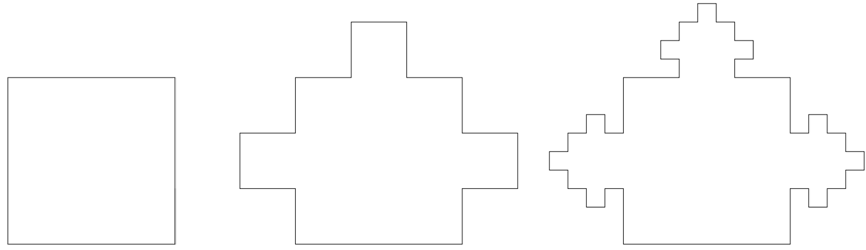
\includegraphics[scale=0.5]{quadratpflanze.png}
			\end{figure}
			\begin{enumerate}[label=\alph*)]
				\item Wird die Fläche unendlich gross? Begründe.
				\item Wird der Umfang unendlich lang? Begründe.
			\end{enumerate}
			\item Ein spiralförmiger Weg beginnt beim Ursprung $(0,0)$ und besteht aus Strecken (wie abgebildet), die eine geometrische Folge bilden.\newline %DMK Ana S12 A73
			\begin{minipage}{0.6\linewidth}
				\begin{enumerate}[label=\alph*)]
					\item Wie lang ist der unendlich fortgesetzte Weg?
					\item Wo liegt der Zielpunkt $Z$ dieses Weges?
				\end{enumerate}
			\end{minipage}
			\hfill
			\begin{minipage}{0.35\linewidth}
				\centering
				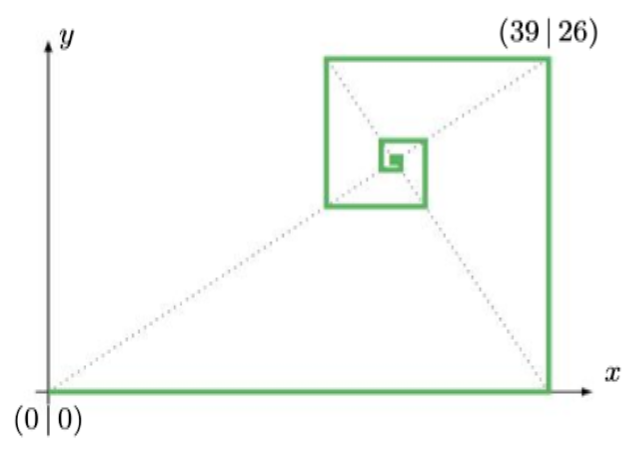
\includegraphics[scale=0.2]{images/spiralweg.png}
			\end{minipage}
		\end{enumerate}
	\end{aufgabe}
	Wir haben also gesehen, dass eine geometrische Folge gegen Null streben kann. Gleichzeitig kann sich die zugehörige Reihe aber einer beliebigen reelen Zahl annähern. Ob dieses Verhalten auch für eine Folge erklärt werden kann und woran wir erkennen, wohin eine Folge konvergiert wird im folgenden Abschnitt erläutert. \newpage


\section{Konvergenz von Folgen}
	Wir lösen uns an dieser Stelle von den zwei Spezialfällen (arithemtisch und geometrisch) und fassen den Begriff der Folge wieder viel breiter. Es müssen also keine Regelmässigkeiten mehr zwischen den einzelnen Folgenglieder vorkommen. Im Zusammenhang mit den unendlichen geometrischen Reihen haben wir den Begriff des Grenzwertes bereits kennengelernt. Dabei ist dieser der Zahlenwert, den die geometrische Reihe nach der Summierung aller unendlich vielen Folgenglieder annimmt. Der Begriff des Grenzwertes kann aber über die Reihen hinaus auch ganz allgemein definiert werden.
	\begin{definition}
		Eine Zahl $g\in\R$ heisst Grenzwert der Folge $(a_n)_{n\in\N}$, wenn die einzelnen Glieder $a_n$ für wachsendes $n$ dem Wert $g$ beliebig nahekommen und beliebig nahe bleiben.\\
		Notation: \[a_n\lto a \text{ für } n\lto\infty \qquad\text{oder}\qquad \lim_{n\to\infty}a_n=g\]
	\end{definition}
	\begin{beispiel}\ \\
		\begin{minipage}{0.5\linewidth}
			Gegen welchen Grenzwert strebt die Folge ${a_n=\frac{1}{n}}$? Erstelle zuerst eine Wertetabelle und stelle die Werte danach im Graphen dar.
			\begingroup
			\renewcommand{\arraystretch}{1.5}
			\begin{table}[H]
				\centering
				\begin{tabular}{c|p{5mm}|p{5mm}|p{5mm}|p{5mm}|p{5mm}|p{5mm}|p{5mm}|p{7mm}}
					$n$ & $1$ & $2$ & $3$ & $5$ & $10$ & $20$ & $50$ & $100$ \\\hline
					$a_n$ & & & & & & & &
				\end{tabular}
			\end{table}
			\endgroup
		\end{minipage}
		\hfill
		\begin{minipage}{0.45\linewidth}
			\centering
			\begin{tikzpicture}[cross/.style={draw, cross out, minimum size=2*(#1-1pt), inner sep=0pt, outer sep=0pt}, x=1cm, y=5cm,
				>=latex,   %Voreinstellung für Pfeilspitzen
				font= \footnotesize, scale=0.65]
				%Raster zeichnen
				\draw [color=gray!50]  [step=10mm] (-0.3,0) grid (9.3,1.1);
				% Achsen zeichnen
				\draw[->,thick] (-0.3,0) -- (9.8,0) node[right, below] {\normalsize $n$};
				\draw[->,thick] (0,-0.1) -- (0,1.15) node[above, left] {\normalsize $a_n$};
				% Achsen beschriften
				\foreach \x/\label in {0.5/1,1/2,1.5/3,2/5,3/10,4/20,6/50,9/100} \draw (\x,-.02) -- (\x,.02) node[below=5pt] {$\label$};
				\foreach \y in {0.2,0.4,0.6,0.8,1} \draw (-.1,\y) -- (.1,\y) node[left=4pt] {$\y$};
				% Besserer Ursprung
				\draw[color=black] (0pt,-14pt) node[left] {$0$};
				%Funktionen zeichnen:
				%\clip(-3.3,-5.3) rectangle (3.3,7.3); %Bildbereich
				%\draw[blue, smooth, domain=-9:9] plot (\x, {-1*pow(\x-3,2)+1}) node[yshift=13cm] {$$};
				%\draw[green, smooth, domain=-9:9] plot (\x, {2*pow(\x-3,2)-3}) node[] {$$};
				%\draw[red, smooth, domain=-9:9] plot (\x, {-0.4*pow(\x+3,2)+1}) node[right] {$$};
				%Beschriftung
				%\node[blue]  at (1,-5) {$p_2$};
			\end{tikzpicture}
		\end{minipage}
		\vspace{7pt}\\\karos{4.5}
	\end{beispiel}
	\begin{aufgabe}
		\label{aufg:grenzwertvermuten}
		Beurteile zu welchem Grenzwert (falls vorhanden), die untenstehenden Folgen konvergieren. Notiere dazu einige Glieder der Folge und stelle eine Vermutung auf.
		\begin{enumcols}[3]
			\item $\ds a_n=\frac{5}{5+n}$
			\item $\ds a_n=\frac{7}{2n-1}$
			\item $\ds a_n=\frac{k-10}{10}$
			\item $\ds a_n=\left(\frac{4}{5}\right)^n$
			\item $\ds a_n=3+\left(\frac{-7}{8}\right)^n$
			\item $\ds a_n=2+\left(\frac{4}{3}\right)^n$
		\end{enumcols}
	\end{aufgabe}\newpage
	Um über solche Dinge präzise sprechen zu können, brauchen wir dringend eine genaue Formulierung dessen, was wir unter einem Grenzwert verstehen wollen. Die nun folgende Definition nennt ein präzises Kriterium dafür, ob eine Folge konvergiert, also einen Grenzwert hat, oder nicht. Da alles Folgende auf einem genauen Verständnis dieser Definition beruht, ist sie sehr wichtig.
	\begin{definition}
		Eine Zahl $g\in\R$ heisst Grenzwert der Folge $(a_n)$ genau dann, wenn zu jeder noch so kleinen positiven Zahl $\epsilon>0$ ein Index $N$ existiert, sodass der Abstand von allen folgenden Folgenglied zum Grenzwert $\abs{a_n-g}<\epsilon$ gilt.
	\end{definition}
	Stellen wir und das ganze bildlich vor: Eine konvergente Folge ist eine, deren Glieder einer bestimmten Zahl $g$ immer näherkommen. So haben wir dies auch bereits in der Aufgabe \thesection.\ref{aufg:grenzwertvermuten}. Die Definition beschreibt dieses \flqq näherkommen\frqq\:wie folgt: Der Abstand von $a_n$ zum Grenzwert $g$ wird mit wachsendem Index $n$ immer kleiner. Betrachte dazu die Abbildung \ref{fig:epsstreifen-grob}. Was heisst das genau:
	\begin{figure}[H]
		\centering
		\begin{tikzpicture}[cross/.style={draw, cross out, minimum size=2*(#1-1pt), inner sep=0pt, outer sep=0pt}, x=1cm, y=1cm,
			>=latex,   %Voreinstellung für Pfeilspitzen
			font= \footnotesize, scale=0.7]
			% Achsen zeichnen
			\draw[->,thick] (-0.3,0) -- (17.8,0) node[right, below] {\normalsize $n$};
			\draw[->,thick] (0,-0.1) -- (0,3.8) node[above, left] {\normalsize $a_n$};
			% Achsen beschriften
			\foreach \x/\label in {0/0,1/1,2/2,3/3,4/\ldots,9/$N$} \draw (\x,-.1) -- (\x,.1) node[below=4pt] {$\label$};
			\foreach \y/\label in {1.3/$g-\epsilon$,2/$g$,2.7/$g+\epsilon$} \draw (-.1,\y) -- (.1,\y) node[left=4pt] {$\label$};
			%Funktionen zeichnen:
			\clip(-0.3,-1.1) rectangle (17.3,4.3); %Bildbereich
			\fill[yellow!30, opacity=0.5] (0,1.3) rectangle (17.3,2.7);
			\draw[black,dashed,smooth,domain=0:17.3] plot (\x, {2.7});
			\draw[black,thick,smooth,domain=0:17.3] plot (\x, {2});
			\draw[black,dashed,smooth,domain=0:17.3] plot (\x, {1.3});
			\foreach \x/\y in {1/0.4,2/0.8,3/1.7,4/2.6,5/3,6/3.2,7/3.05,8/2.8,9/2.55,10/2.2,11/1.8,12/1.6,13/2.05,14/1.95,15/1.98,16/2.07,17/1.99,18/2.01}{\fill[forestgreen] (\x,\y) circle (2pt);} % Folgepunkte
			% Beschriftung
			\node[above] at (15,3.5) {Streifen der Breite $\epsilon$};
			\draw[->] (15,3.5) -- (14.3,2.75);
			% Box als Ausschnitt für zweiten Graph
			\draw[plotblue,line width=2pt] (7.5,-0.8) rectangle (12.5,3.2);
		\end{tikzpicture}
		\caption{Möglicher Graph einer konvergierenden Folge}
		\label{fig:epsstreifen-grob}
	\end{figure}
	Wenn wir eine (noch so) kleine Zahl $\epsilon>0$ vorgeben, ab irgendeinem bestimmten Index werden die Abstände der Folgeglieder zu $g$ immer kleiner sein als diese vorgegebene Zahl. Dieser Übergang ist in der Abbildung \ref{fig:epsstreifen-fein} sehr schön veranschaulicht. Der Betrag brauchen wir, weil sich die Folgenglieder an gewissenstellen auch unterhalb des Grenzwerts liegen können. Betrachten wir die
	\begin{figure}[H]
		\centering
		\begin{tikzpicture}[cross/.style={draw, cross out, minimum size=2*(#1-1pt), inner sep=0pt, outer sep=0pt}, x=1cm, y=1cm,
			>=latex,   %Voreinstellung für Pfeilspitzen
			font= \footnotesize, scale=1]
			% Achsen zeichnen
			\draw[->,thick] (3.5,0) -- (12.8,0) node[right, below] {\normalsize $n$};
			%\draw[->,thick] (0,-0.1) -- (0,3.8) node[above, left] {\normalsize $a_n$};
			% Achsen beschriften
			\foreach \x/\label in {6/$N$} \draw (\x,-.1) -- (\x,.1) node[below=4pt] {$\label$};
			%\foreach \y/\label in {1.3/$g-\epsilon$,2/$g$,2.7/$g+\epsilon$} \draw (-.1,\y) -- (.1,\y) node[left=4pt] {$\label$};
			%Funktionen zeichnen:
			\clip(3,-0.8) rectangle (13,4.6); %Bildbereich
			\fill[yellow!30, opacity=0.5] (3.5,0.6) rectangle (12.5,3.4);
			\draw[black,dashed,smooth,domain=3.5:12.5] plot (\x, {3.4});
			\draw[black,thick,smooth,domain=3.5:12.5] plot (\x, {2});
			\draw[black,dashed,smooth,domain=3.5:12.5] plot (\x, {0.6});
			\foreach \x/\y in {4/3.6,6/3.1,8/2.4,10/1.6,12/1.2}{\fill[forestgreen] (\x,\y) circle (2pt);} % Folgepunkte
			% Beschriftung
			\draw[myred, <->, thick] (4,2) -- (4,3.6) node[midway,right] {$\abs{a_n-g}>\epsilon$};
			\draw[black, <->, thick] (6,2) -- (6,3.1) node[midway,right] {$\abs{a_n-g}<\epsilon$};
			\draw[black, thick] (6,2) -- (6,0);
			\draw[black, <->, thick] (8,2) -- (8,2.4);
			% Box als Ausschnitt für zweiten Graph
			\draw[plotblue,line width=2pt] (3.5,-0.6) rectangle (12.5,4.4);
		\end{tikzpicture}
		\caption{Vergrösserter Ausschnitt des interessanten Bereichs des obigen Graphen}
		\label{fig:epsstreifen-fein}
	\end{figure}
	So technisch diese Definition ausschauen mag, sie hat riesige Vorteile: Sie konkretisiert unsere bis anhin eher vage Vorstellung eines \flqq Hinstrebens\frqq. Und wir können nun streng beweisen, dass eine bestimmte Zahl der Grenzwert einer bestimmten Folge ist. Es gibt diesbezüglich keine Unklarheiten mehr. Betrachten wir sogleich ein paar einfache Beispiele:
	\begin{beispiel}
		Betrachte dir Folge $\ds a_n=\frac{2n}{n+1}$.\\
		\begin{minipage}{0.5\linewidth}
			\begin{enumerate}[label=\alph*)]
				\item Erstelle zuerst eine Wertetabelle und skizziere die Folge in einem Koordinatensystem.
			\end{enumerate}
			\begingroup
			\renewcommand{\arraystretch}{1.5}
			\begin{table}[H]
				\centering
				\begin{tabular}{c|p{5mm}|p{5mm}|p{5mm}|p{5mm}|p{5mm}|p{5mm}|p{5mm}|p{7mm}}
					$n$ & $1$ & $2$ & $3$ & $5$ & $10$ & $20$ & $50$ & $100$ \\\hline
					$a_n$ & & & & & & & &
				\end{tabular}
			\end{table}
			\endgroup
		\end{minipage}
		\hfill
		\begin{minipage}{0.45\linewidth}
			\centering
			\begin{tikzpicture}[cross/.style={draw, cross out, minimum size=2*(#1-1pt), inner sep=0pt, outer sep=0pt}, x=1cm, y=2cm,
				>=latex,   %Voreinstellung für Pfeilspitzen
				font= \footnotesize, scale=0.65]
				%Raster zeichnen
				\draw [color=gray!50]  [step=10mm] (-0.3,0) grid (9.3,2.6);
				% Achsen zeichnen
				\draw[->,thick] (-0.3,0) -- (9.8,0) node[right, below] {\normalsize $n$};
				\draw[->,thick] (0,-0.1) -- (0,2.8) node[above, left] {\normalsize $a_n$};
				% Achsen beschriften
				\foreach \x/\label in {0.5/1,1/2,1.5/3,2/5,3/10,4/20,6/50,9/100} \draw (\x,-.05) -- (\x,.05) node[below=5pt] {$\label$};
				\foreach \y in {0.5,1,1.5,2,2.5} \draw (-.1,\y) -- (.1,\y) node[left=4pt] {$\y$};
				% Besserer Ursprung
				\draw[color=black] (0pt,-14pt) node[left] {$0$};
				%Funktionen zeichnen:
				%\clip(-3.3,-5.3) rectangle (3.3,7.3); %Bildbereich
				%\draw[blue, smooth, domain=-9:9] plot (\x, {-1*pow(\x-3,2)+1}) node[yshift=13cm] {$$};
			\end{tikzpicture}
		\end{minipage}
		\begin{enumerate}[label=\alph*)]
			\setcounter{enumi}{1}
			\item Ich fixiere $\epsilon=10^{-3}$. Ab welchem Folgenglied $a_n$ ist der Abstand zum Grenzwert $g$ kleiner als der schmale Streifen?
			\item Nun wird $\epsilon=10^{-9}$ fixiert. Gibt es nach wie vor ein Index $N$, sodass der Abstand aller folgenden Folgenglieder kleiner ist als $\epsilon$? Berechne diesen Index.
		\end{enumerate}
		\karos{4.5}
	\end{beispiel}
	\begin{beispiel}\ \\
		\begin{enumerate}[label=\alph*)]
			\item Betrachte die Folge $\ds a_n=2-\frac{(-1)^n}{n}$. Zu welchem Grenzwert konvergiert diese Folge?
			\item Wie breit muss der Streifen gewählt werden, damit alle Folgenglieder mit Index $n>100$ innerhalb des Streifens liegen?
		\end{enumerate}
		\karos{6.5}
	\end{beispiel}
	\begin{aufgabe}
		\begin{enumerate}
			\item Bestimme den Grenzwert $g$ der Folge $(a_n)$ und berechne den kleinsten Index $N$, ab dem alle Folgenglieder weniger als $0.01$ von $g$ entfernt sind.
			\begin{enumcols}[2]
				\item $\ds a_n=\frac{1}{n(n+1)}$
				\item $\ds a_n=2^{-n^2}$
			\end{enumcols}
			\item Ab welchem Index $N$ sind alle Folgenglieder weniger als $10^{-3}$ vom Grenzwert der Folge $(a_n)$ entfernt?
			\begin{enumcols}[3]
				\item $\ds a_n=1+\frac{1}{n}$
				\item $\ds a_n=7-\frac{1}{\sqrt{n}}$
				\item $\ds a_n=\frac{n}{n+1}$
			\end{enumcols}
			\item Entscheide für die folgenden Aussagen, ob sie wahr oder falsch sind.
			\begin{enumerate}[label=\alph*)]
				\item Ist die Folge $a_n=(-1)^n$ konvergent?
				\item Ist die konstante Folge $a_n=4$ konvergent?
				\item Gibt es konvergente arithmetische Folgen?
				\item Gibt es konvergente geometrische Folgen?
			\end{enumerate}
			\item Wie breit muss der Streifen gewählt werden, damit alle Folgenglieder mit Index $n>50$ innerhalb des Streifens liegen?
			\begin{enumcols}[3]
				\item $\ds a_n=\frac{5n-1}{n}$
				\item $\ds a_n=3+\frac{2n}{n^2-1}$
				\item $\ds a_n=\frac{\sqrt{n}}{n}$
			\end{enumcols}
		\end{enumerate}
	\end{aufgabe}\newpage


\section{Grenzwertsätze}
	\begin{aufgabe}
		Wir haben schon gesehen, dass $\lim_{n\to\infty}\left(\frac{1}{n}\right)=0$, dass eine konstante Folge konvergiert und das $\lim_{n\to\infty}\left(\frac{n}{n+1}\right)=1$ ist. Wie kannst du dieses Wissen benutzen, um die folgenden Grenzwerte einfach und elegant auszurechnen?
		\begin{enumcols}[3]
			\item $\ds\lim_{n\to\infty}\left(\frac{1}{n}+5\right)$
			\item $\ds\lim_{n\to\infty}\left(3.7-\frac{1}{n}\right)$
			\item $\ds\lim_{n\to\infty}\left(13\*\frac{n}{n+1}\right)$
			\item $\ds\lim_{n\to\infty}\left(\frac{n}{n+1}+\frac{1}{n}\right)$
			\item $\ds\lim_{n\to\infty}\left(\left(2+\frac{1}{n}\right)\*\left(6-\frac{1}{n}\right)\right)$
			\item $\ds\lim_{n\to\infty}\left(\frac{4+\frac{1}{n}}{8+\frac{1}{n}}\right)$
		\end{enumcols}
		Welche Gesetzmässigkeiten über Grenzwerte hast du hier intuitiv und automatisch verwendet?\vspace{7pt}\\\karos{4.5}
	\end{aufgabe}
	Nun steht also die Vermutung im Raum, dass Grenzwerte die vier Grundrechenarten respekieren und somit die Terme aus der obigen Aufgabe auseinander genommen und einzeln berechnet werden dürfen. Dies müssten wir an dieser Stelle aber explizit beweisen.
	\begin{satz}
		Gegeben sind zwei konvergente Folgen $(a_n)$ und $(b_n)$ mit den jeweiligen Grenzwerten ${\ds\lim_{n\to\infty}(a_n)=g}$ und $\ds\lim_{n\to\infty}(b_n)=h$.\\ Die Summe der beiden Folgen $c_n:=a_n+b_n$ ist ebenfalls eine konvergente Folge und sie besitzt den Grenzwert \[\lim_{n\to\infty}(c_n)=\lim_{n\to\infty}(a_n)+\lim_{n\to\infty}(b_n)=g+h.\]
	\end{satz}
	\begin{beweis}
		Wir wählen ein beliebig kleines $\epsilon>0$. Jetzt müssen wir zeigen, dass es einen Index $N$ gibt, sodass der Abstand von $c_n$ zur Summe der beiden Grenzwerte von $a_n$ und $b_n$ kleiner ist als $\epsilon$ für $n>N$; i.e. $\ds\abs{c_n-(g+h)}<\epsilon$.\\
		Da die Folge $a_n$ zum Grenzwert $g$ konvergiert, existiert für diese Folge sicherlich einen Index $N_a$, sodass \vspace{7pt}\\\karos{1.5}
		Da die Folge $b_n$ zum Grenzwert $h$ konvergiert, existiert für diese Folge sicherlich einen Index $N_b$, sodass \vspace{7pt}\\\karos{1.5}
		Dann gilt gür alle $n>N:=\max{N_a,N_b}$, dass \vspace{7pt}\\\karos{4.5}
	\end{beweis}
	Die genau gleiche Argumentation kann für jede andere Grundrechenart herangezogen werden und damit können wir uns also sicher sein, dass die folgenden Grenzwertsätze für alle Operationen (Addition, Subtraktion, Multiplikation und Division) gelten.
	\begin{satz}[Grenzwertsätze]
		\label{satz:grenzwertsaetze}
		Gegeben sind zwei konvergente Folgen $(a_n)$ und $(b_n)$, dann gilt:
		\begin{enumerate}[label=\ ,leftmargin=2cm]
			\item $\ds\lim_{n\to\infty}\left(a_n\pm b_n\right)=$
			\item $\ds\lim_{n\to\infty}\left(a_n\* b_n\right)=$
			\item $\ds\lim_{n\to\infty}\left(\frac{a_n}{b_n}\right)=$
		\end{enumerate}
		Zudem können wir ganz allgemein formulieren:
		\begin{enumerate}[label=\ ,leftmargin=2cm]
			\item Gilt $\ds\lim_{n\to\infty}\left(a_n\right)=\infty\quad\Rightarrow$
		\end{enumerate}
	\end{satz}
	Damit haben wir eine Mothode entwickelt, wie man Grenzwerte analytisch berechnen kann (also nicht durch Einsetzen und Bauchgefühl). Als erstes Beispiel betrachten wir also
	\begin{beispiel}
		Gegeben ist die Folge $\ds a_n=\frac{10n-2n^2}{n^2+5}$. Berechne $\ds\lim_{n\to\infty}(a_n)$.\vspace{7pt}\\\karos{4.5}
	\end{beispiel}
	\begin{beispiel}
		Gegeben ist die Folge $\ds a_n=\frac{10n^2-4n+1}{n^3+3n+4}$. Berechne $\ds\lim_{n\to\infty}(a_n)$.\vspace{7pt}\\\karos{4.5}
	\end{beispiel}
	\begin{aufgabe}
			Die Folge $(a_n)$ ist durch das allgemeine Glied gegeben. Berechne für jede Folge $\ds\lim_{n\to\infty}(a_n)$.
			\begin{enumcols}[3]
				\item $\ds\lim_{n\to\infty}\left(\frac{2n^2-4n}{n^2+3n-5}\right)$
				\item $\ds\lim_{n\to\infty}\left(\frac{3n-21}{4n^2}\right)$
				\item $\ds\lim_{n\to\infty}\left(\frac{n^2}{5n^2+n}\right)$
				\item $\ds\lim_{n\to\infty}\left(\frac{(-1)^n\*8}{n^2+1}\right)$
				\item $\ds\lim_{n\to\infty}\left(\frac{4n+3\*(-1)^n}{2n}\right)$
				\item $\ds\lim_{n\to\infty}\left(\frac{(2n-1)^3}{(n-1)^3}\right)$
				\item $\ds\lim_{n\to\infty}\left(\frac{1-n^2}{n}\right)$
				\item $\ds\lim_{n\to\infty}\left(\frac{3n^7-4n^5}{2n^7+7n^6}\right)$
				\item $\ds\lim_{n\to\infty}\left(\frac{3-n^3}{2n^3+n^2}\right)$
			\end{enumcols}
	\end{aufgabe}
	\begin{aufgabe}[für Schnelle]
		\begin{enumerate}
			\item Gegeben ist die Folge $\ds a_n=\frac{4n^4-6n^3+7}{2n^m+5n+1}$.\vspace{2pt}\\Bestimme den Exponenten $m\in\N_0$ so, dass die folgenden Grenzwerte resultieren, oder erkläre, weshalb es kein $m$ mit diesem Grenzwert gibt.
			\begin{enumcols}[3]
				\item $\ds\lim_{n\to\infty}(a_n)=2$
				\item $\ds\lim_{n\to\infty}(a_n)=0$
				\item $\ds\lim_{n\to-\infty}(a_n)=-2$
				\item $\ds\lim_{n\to-\infty}(a_n)=-\infty$
				\item $\ds\lim_{n\to-\infty}(a_n)=\infty$
			\end{enumcols}
			\item Berechne.
			\begin{enumcols}[3]
				\item $\ds\lim_{n\to\infty}\left(\frac{n^3+\sin{n}}{n^3}\right)$
				\item $\ds\lim_{n\to-\infty}\left(\frac{n^2-\sin{n}}{n^3}\right)$
				\item $\ds\lim_{n\to\infty}\left(\frac{\cos{n}-3n}{1-2n}\right)$
			\end{enumcols}
		\end{enumerate}
	\end{aufgabe}\newpage


\section{Konvergenz von Funktionen}
	Bevor wir in diesem Abschnitt das Augenmerk von Folgen auf Funktionen schwenken, lasst uns zuerst einen Vergleich anstellen und den Unterschied resp. die Gemeinsamkeiten einer Folge und einer Funktion diskutieren. Dazu untersuchen wir den Funktionsverlauf der Funktion $f(x)$ und der Folge $a_n$ auf der positiven reelen Achse.\\
	\begin{minipage}[t]{0.28\linewidth}
		\centering
		\[f(x)=\frac{2x+6}{x+1}\]\vspace{5pt}
		\[a_n=\frac{2n+6}{n+1}\]
	\end{minipage}
	\begin{minipage}[t]{0.68\linewidth}
		\centering
		\vspace{8pt}
		\begin{tabular}{c|p{5mm}|p{5mm}|p{5mm}|p{5mm}|p{5mm}|p{5mm}|p{5mm}|p{7mm}|p{8mm}}
			$n$ & $0$ & $0.5$ & $1$ & $2$ & $5$ & $10$ & $50$ & $100$ & $1000$ \\\hline
			$\:\: a_n \:\:$ & & & & & & & & &
		\end{tabular}\vspace{20pt}\\
		\begin{tabular}{c|p{5mm}|p{5mm}|p{5mm}|p{5mm}|p{5mm}|p{5mm}|p{5mm}|p{7mm}|p{8mm}}
			$x$ & $0$ & $0.5$ & $1$ & $2$ & $5$ & $10$ & $50$ & $100$ & $1000$ \\\hline
			$f(x)$ & & & & & & & & &
		\end{tabular}
	\end{minipage}\vspace{5pt}\\
	{\bf Graph:}
	\begin{figure}[H]
		\centering
		\begin{tikzpicture}[cross/.style={draw, cross out, minimum size=2*(#1-1pt), inner sep=0pt, outer sep=0pt}, x=1cm, y=1cm,
			>=latex,   %Voreinstellung für Pfeilspitzen
			font= \footnotesize, scale=0.65]
			%Raster zeichnen
			\draw [color=gray!50]  [step=10mm] (0,0) grid (15.3,6.3);
			% Achsen zeichnen
			\draw[->,thick] (-0.3,0) -- (15.8,0) node[right, below] {\normalsize $x,n$};
			\draw[->,thick] (0,-0.3) -- (0,6.8) node[above, left] {\normalsize $y$};
			% Achsen beschriften
			\foreach \x in {1,2,...,15} \draw (\x,-.1) -- (\x,.1) node[below=4pt] {$\x$};
			\foreach \y in {1,2,...,6} \draw (-.1,\y) -- (.1,\y) node[left=4pt] {$\y$};
			% Besserer Ursprung
			\draw[color=black] (0pt,-14pt) node[left] {$0$};
			%Funktionen zeichnen:
			%\clip(-3.3,-5.3) rectangle (3.3,7.3); %Bildbereich
			%\draw[blue, smooth, domain=-9:9] plot (\x, {-1*pow(\x-3,2)+1}) node[yshift=13cm] {$$};
		\end{tikzpicture}
	\end{figure}
	{\bf Feststellung:}\vspace{2pt}\\\karos{3.5}

\subsection{Grenzwerte im Unendlichen}
	\begin{beispiel}\ \\
		\begin{minipage}{0.475\linewidth}
			{\bf Potenzfunktionen:}
			\centering
			\begin{tikzpicture}[cross/.style={draw, cross out, minimum size=2*(#1-1pt), inner sep=0pt, outer sep=0pt}, x=1cm, y=1cm,
				>=latex,   %Voreinstellung für Pfeilspitzen
				font= \footnotesize, scale=0.65]
				%Raster zeichnen
				\draw [color=gray!50]  [step=10mm] (-5.3,-3.3) grid (5.3,3.3);
				% Achsen zeichnen
				\draw[->,thick] (-5.3,0) -- (5.8,0) node[right, below] {\normalsize $x$};
				\draw[->,thick] (0,-3.3) -- (0,3.8) node[above, left] {\normalsize $y$};
				% Achsen beschriften
				\foreach \x in {-5,...,-3,-2,-1,1,2,...,5} \draw (\x,-.1) -- (\x,.1) node[below=4pt] {$\x$};
				\foreach \y in {-3,-2,-1,1,2,...,3} \draw (-.1,\y) -- (.1,\y) node[left=4pt] {$\y$};
				% Besserer Ursprung
				\draw[color=black] (0pt,-8pt) node[right] {$0$};
				%Funktionen zeichnen:
				\clip(-5.3,-3.3) rectangle (5.3,3.3); %Bildbereich
				\draw[plotblue, thick, domain=-5.3:5.3, samples=100] plot (\x, {pow(\x,2)});
				\draw[highdive, thick, domain=-5.3:-0.01, samples=200] plot (\x, {pow(\x,-1)});
				\draw[highdive, thick, domain=0.01:5.3, samples=200] plot (\x, {pow(\x,-1)}) node[above=8pt,left=4pt] {$x^{-1}$};
				\draw[plotblue] (2,2.8) node {$x^2$};
			\end{tikzpicture}
		\end{minipage}
		\hfill
		\begin{minipage}{0.475\linewidth}
			{\bf $\log{}-$ \& $\exp{}-$ Funktionen:}
			\centering
			\begin{tikzpicture}[cross/.style={draw, cross out, minimum size=2*(#1-1pt), inner sep=0pt, outer sep=0pt}, x=1cm, y=1cm,
				>=latex,   %Voreinstellung für Pfeilspitzen
				font= \footnotesize, scale=0.65]
				%Raster zeichnen
				\draw [color=gray!50]  [step=10mm] (-5.3,-3.3) grid (5.3,3.3);
				% Achsen zeichnen
				\draw[->,thick] (-5.3,0) -- (5.8,0) node[right, below] {\normalsize $x$};
				\draw[->,thick] (0,-3.3) -- (0,3.8) node[above, left] {\normalsize $y$};
				% Achsen beschriften
				\foreach \x in {-5,...,-2,-1,1,2,...,5} \draw (\x,-.1) -- (\x,.1) node[below=4pt] {$\x$};
				\foreach \y in {-3,-2,-1,1,2,...,3} \draw (-.1,\y) -- (.1,\y) node[left=4pt] {$\y$};
				% Besserer Ursprung
				\draw[color=black] (0pt,-8pt) node[right] {$0$};
				%Funktionen zeichnen:
				\clip(-5.3,-3.3) rectangle (5.8,3.3); %Bildbereich
				\draw[plotblue, thick, domain=-5.3:5.3, samples=100] plot (\x, {exp(\x)});
				\draw[plotblue] (1.4,2.8) node {$\exp{x}$};
				\draw[highdive, thick, domain=0.01:5.3, samples=100] plot (\x, {ln(\x)});
				\draw[highdive] (5,1.1) node {$\ln{x}$};
			\end{tikzpicture}
		\end{minipage}\vspace{4pt}\\
		\begin{minipage}{0.475\linewidth}
			{\bf Trigonometrische Funktionen:}
			\centering
			\begin{tikzpicture}[cross/.style={draw, cross out, minimum size=2*(#1-1pt), inner sep=0pt, outer sep=0pt}, x=1cm, y=1cm,
				>=latex,   %Voreinstellung für Pfeilspitzen
				font= \footnotesize, scale=0.65]
				%Raster zeichnen
				\draw [color=gray!50]  [step=10mm] (0,-3.3) grid (10.3,3.3);
				% Achsen zeichnen
				\draw[->,thick] (-0.3,0) -- (10.8,0) node[right, below] {\normalsize $x$};
				\draw[->,thick] (0,-3.3) -- (0,3.8) node[above, left] {\normalsize $y$};
				% Achsen beschriften
				\foreach \x in {1,2,...,10} \draw (\x,-.1) -- (\x,.1) node[below=4pt] {$\x$};
				\foreach \y in {-3,-2,-1,0,1,2,...,3} \draw (-.1,\y) -- (.1,\y) node[left=4pt] {$\y$};
				% Besserer Ursprung
				%\draw[color=black] (0pt,-8pt) node[left] {$0$};
				%Funktionen zeichnen:
				\clip(0,-3.3) rectangle (10.3,3.3); %Bildbereich
				\draw[plotblue, thick, domain=0:10.3, samples=500] plot (\x, {sin(2*\x r)}) node[above=6pt,left=4pt] {$f$};
			\end{tikzpicture}
		\end{minipage}
		\hfill
		\begin{minipage}{0.475\linewidth}
			\centering
			\begin{tikzpicture}[cross/.style={draw, cross out, minimum size=2*(#1-1pt), inner sep=0pt, outer sep=0pt}, x=1cm, y=1cm,
				>=latex,   %Voreinstellung für Pfeilspitzen
				font= \footnotesize, scale=0.65]
				%Raster zeichnen
				\draw [color=gray!50]  [step=10mm] (0,-3.3) grid (10.3,3.3);
				% Achsen zeichnen
				\draw[->,thick] (-0.3,0) -- (10.8,0) node[right, below] {\normalsize $x$};
				\draw[->,thick] (0,-3.3) -- (0,3.8) node[above, left] {\normalsize $y$};
				% Achsen beschriften
				\foreach \x in {1,2,...,10} \draw (\x,-.1) -- (\x,.1) node[below=4pt] {$\x$};
				\foreach \y in {-3,-2,-1,0,1,2,...,3} \draw (-.1,\y) -- (.1,\y) node[left=4pt] {$\y$};
				% Besserer Ursprung
				%\draw[color=black] (0pt,-8pt) node[left] {$0$};
				%Funktionen zeichnen:
				\clip(0,-3.3) rectangle (10.3,3.3); %Bildbereich
				\draw[plotblue, thick, domain=0:10.3, samples=500] plot (\x, {3*exp(-0.2*\x)*cos(2*\x r)}) node[above=14pt,left=4pt] {$f$};
			\end{tikzpicture}
		\end{minipage}
	\end{beispiel}
	Wir können also an dieser Stelle festhalten, dass für die Diskussion von Grenzwerte von Funktionen die genau gleichen \flqq Regeln\frqq\:wie für die Folgen gelten. Entsprechend können wir den Satz \ref{satz:grenzwertsaetze} wie folgt auf die Funktionen erweitern.
	\begin{satz}[Grenzwertsätze]
		Gegeben sind zwei Funktionen $f$ und $g$ mit je einem Grenzwert $\ds\lim_{x\to\infty}f(x)$ und $\ds\lim_{x\to\infty}g(x)$, dann gilt:
		\begin{enumerate}[label=\ ,leftmargin=2cm]
			\item $\ds\lim_{n\to\infty}\left(f\pm g\right)=$
			\item $\ds\lim_{n\to\infty}\left(f\* g\right)=$
			\item $\ds\lim_{n\to\infty}\left(\frac{f}{g}\right)=$
		\end{enumerate}
		Zudem können wir ganz allgemein formulieren:
		\begin{enumerate}[label=\ ,leftmargin=2cm]
			\item Gilt $\ds\lim_{n\to\infty}\left(f\right)=\infty\quad\Rightarrow$
		\end{enumerate}
	\end{satz}
	Das heisst im Allgemeinen können damit weitere Grenzwerte von Funktionen berechnen.
	\begin{aufgabe}
		\begin{enumerate}
			\item Die Folge $(a_n)$ ist durch das allgemeine Glied gegeben. Berechne für jede Folge $\ds\lim_{n\to\infty}(a_n)$.
			\begin{enumcols}[3]
				\item $\ds\lim_{x\to\infty}\left(\frac{3x-1}{x+2}\right)$
				\item $\ds\lim_{x\to\infty}\left(\frac{3x+1}{x^2}\right)$
				\item $\ds\lim_{x\to\infty}\left(\frac{3-x^2}{x^4-2x^2}\right)$
				\item $\ds\lim_{x\to\infty}\left(\frac{8x^3}{2x^2+x}\right)$
				\item $\ds\lim_{x\to\infty}\left(\frac{4x+3}{2x^6}\right)$
				\item $\ds\lim_{x\to\infty}\left(\frac{x^4+x^2+6}{9-x^4}\right)$
			\end{enumcols}
			\item Bestimme die Parameter $a$,$b$ und $c$ so, dass gilt: \[\lim_{x\to\infty}\left(\frac{a\*x^b+4x^5+c\*x^3-1}{2x^3-11x^2+5}\right)=3\]
		\end{enumerate}
	\end{aufgabe}

\subsection{Grenzwerte im Endlichen}
	Betrachte dir die Funktion $\ds f(x)=\frac{2x^2+x}{x}$.\\
	\begin{minipage}{0.575\linewidth}
		\begin{enumerate}[label=\alph*)]
			\item Erstelle zuerst eine Wertetabelle und skizziere die Folge in einem Koordinatensystem.
		\end{enumerate}
		\begingroup
		\renewcommand{\arraystretch}{1.5}
		\begin{table}[H]
			\centering
			\begin{tabular}{c|p{5mm}|p{5mm}|p{5mm}|p{5mm}|p{5mm}|p{5mm}|p{5mm}|p{7mm}}
				$x$ & $1$ & $2$ & $3$ & $5$ & $10$ & $20$ & $50$ & $100$ \\\hline
				$f(x)$ & & & & & & & &
			\end{tabular}
		\end{table}
		\endgroup
	\end{minipage}
	\hfill
	\begin{minipage}{0.4\linewidth}
		\centering
		\begin{tikzpicture}[cross/.style={draw, cross out, minimum size=2*(#1-1pt), inner sep=0pt, outer sep=0pt}, x=1cm, y=1cm,
			>=latex,   %Voreinstellung für Pfeilspitzen
			font= \footnotesize, scale=0.7]
			%Raster zeichnen
			\draw [color=gray!50]  [step=10mm] (-3.3,-3.3) grid (5.3,3.3);
			% Achsen zeichnen
			\draw[->,thick] (-3.3,0) -- (5.8,0) node[right, below] {\normalsize $x$};
			\draw[->,thick] (0,-3.3) -- (0,3.8) node[above, left] {\normalsize $y$};
			% Achsen beschriften
			\foreach \x in {-3,...,-2,-1,1,2,...,5} \draw (\x,-.1) -- (\x,.1) node[below=5pt] {$\x$};
			\foreach \y in {-3,...,-2,-1,1,2,...,3} \draw (-.1,\y) -- (.1,\y) node[left=4pt] {$\y$};
			% Besserer Ursprung
			\draw[color=black] (0pt,-10pt) node[right] {$0$};
			%Funktionen zeichnen:
			%\clip(-3.3,-5.3) rectangle (3.3,7.3); %Bildbereich
			%\draw[blue, smooth, domain=-9:9] plot (\x, {-1*pow(\x-3,2)+1}) node[yshift=13cm] {$$};
		\end{tikzpicture}
	\end{minipage}\vspace{6pt}\\
	Der Grenzwert dieser Funktion im unendlichen ist nicht interessant, da die Funktionswerte immer grösser und grösser werden und die Funktion somit für $x\lto\infty$ divergiert.\\
	\begin{minipage}{0.575\linewidth}
		Allerdings ist die Funktion \gap{4} für $x_0=0$. Nähern wir uns mit $x$ gegen diese Stelle $0$, nähern sich die Funktionswerte beliebig nahe der Zahl $1$.\\ Auch hier sagen wir, die Funktion \gap{3} für $x\lto x_0$ gegen den Grenzwert $1$.\\
	\end{minipage}
	\hfill
	\begin{minipage}{0.4\linewidth}
		\ \vspace{3.2cm}\\
	\end{minipage}
	Geschrieben wird das ebenfalls analog zu den Folgen:\vspace{6pt}\\\karos{2.5}
	\begin{definition}[Definitionslücke]
		Ist eine Funktion $f$ an einer Stelle $x_0$ nicht definitiert, so wird diese Stelle als \textbf{Definitionslücke} bezeichnet.
	\end{definition}
	Diese Definitionslücke $x_0=0$ in der Funktion $f(x)=\frac{2x^2+x}{x}$ erkennen wir auch in der Funktionsgleichung, denn sobald die Zahl $0$ eingesetzt wird, wird der Bruch durch $0$ geteilt, was bekanntlich nicht erlaubt ist. Damit teilt die Definitionslücke unseren Funktionsgraphen in einen linken und einen rechten Teil. Wir können uns also von beiden Seiten her dieser Stelle nähern. Dementsprechend gibt es auch zwei verschiedene Grenzwerte; einen von der linken Seite kommend und den zweiten von der rechten Seite herkommend.
	\begin{definition}
		Der Grenzwert \gap{4} heisst rechtsseitiger Grenzwert und \gap{4} heisst linksseitiger Grenzwert.
	\end{definition}
	Wie wir im Einsteigsbeispiel mit der Funktion $f(x)=\frac{2x^2+x}{x}$ gesehen haben, können die beiden Grenzwerte übereinstimmen. Dies hängt aber stark von der Funktion ab und gilt nicht allgemein.
	\begin{beispiel}
		Wir untersuchen die Funktion $f(x)=\frac{1}{x-1}$ an der Stelle $x_0=1$. Nähern wir uns von der linken Seite an die Stelle $x_0$ an, gehen die Funktionswerte immer weiter ins Negative. Nähern wir uns von der rechten Seite gehen wir genau in entgegengesetzte Richtung; also werden die Funktionswerte immer grösser im Positiven.\\
		\begin{minipage}{0.5\linewidth}
			\centering
			\begin{tikzpicture}[cross/.style={draw, cross out, minimum size=2*(#1-1pt), inner sep=0pt, outer sep=0pt}, x=1cm, y=1cm,
				>=latex,   %Voreinstellung für Pfeilspitzen
				font= \footnotesize, scale=0.7]
				%Raster zeichnen
				\draw [color=gray!50]  [step=10mm] (-5.3,-3.3) grid (5.3,3.3);
				% Achsen zeichnen
				\draw[->,thick] (-5.3,0) -- (5.8,0) node[right, below] {\normalsize $x$};
				\draw[->,thick] (0,-3.3) -- (0,3.8) node[above, left] {\normalsize $y$};
				% Achsen beschriften
				\foreach \x in {-5,...,-2,-1,1,2,...,5} \draw (\x,-.1) -- (\x,.1) node[below=5pt] {$\x$};
				\foreach \y in {-3,...,-2,-1,1,2,...,3} \draw (-.1,\y) -- (.1,\y) node[left=4pt] {$\y$};
				% Besserer Ursprung
				\draw[color=black] (0pt,-10pt) node[right] {$0$};
				%Funktionen zeichnen:
				%\clip(-3.3,-3.3) rectangle (3.3,3.3); %Bildbereich
				%\draw[blue, thick, domain=-3.3:0.99, samples=200] plot (\x, {1/(\x-1)});
				%\draw[blue, thick, domain=1.01:3.3, samples=200] plot (\x, {1/(\x-1)});
			\end{tikzpicture}
		\end{minipage}
		\hfill
		\begin{minipage}{0.475\linewidth}
			\begin{enumerate}[label=\ ]
				\item $\ds\lim_{x\to1^-}f(x)=$
				\item
				\item $\ds\lim_{x\to1^+}f(x)=$
			\end{enumerate}
		\end{minipage}
	\end{beispiel}
	\begin{itemize}
		\item Der Grenzwert einer Funktion an der Stelle $x_0$ existiert nur, wenn der linksseite und rechtsseitige Grenzwert übereinstimmen. In diesem Fall können wir den Grenzwert wie folgt angeben:
		\begin{enumerate}[label=\ ,leftmargin=2cm]
			\item $\ds\lim_{x\to x_0^-}f(x)=\lim_{x\to x_0^+}f(x)=$
		\end{enumerate}
		\item Sind der links- und rechtsseitige Grenzwert nicht gleich, so existiert der Grenzwert nicht.
		\begin{enumerate}[label=\ ,leftmargin=2cm]
			\item $\ds\lim_{x\to x_0^-}f(x)\neq\lim_{x\to x_0^+}f(x)$
		\end{enumerate}
	\end{itemize}
	Da wir hier die Variable $x$ nicht einfach gegen $\infty$ schicken, können wir für die Berechnung des Grenzwertes nicht auch unsere bekannten Methoden zurückgreifen. Da die gesuchte Stelle aber eine reele Zahl ist ($x_0\in\R$), kann der Grenzwert durch einsetzen der entsprechenden Zahl berechnet werden.
	\begin{beispiel}
		Berechne den Grenzwert $\ds\lim_{x\to 5}\left(\frac{x-1}{x^2-1}\right)$.\vspace{5pt}\\\karos{2.5}
	\end{beispiel}
	Leider ist das Einsetzen der Zahl nicht immer möglich. In diesem Fall ist ein zusätzlicher Umformungsschritt notwendig.
	\begin{beispiel}
		Berechne den Grenzwert $\ds\lim_{x\to 2}\left(\frac{x^3-3x-2}{x^2-4}\right)$.\vspace{5pt}\\\karos{4.5}
	\end{beispiel}
	\begin{aufgabe}
		\begin{enumerate}
			\item Betrachte den Ausschnitt des Graphen einer Funktion $f$. Welche Vermutungen bezüglich der folgenden Grenzwerte ergeben sich daraus?\\
			\begin{minipage}{0.6\linewidth}
				\centering
				\begin{tikzpicture}[cross/.style={draw, cross out, minimum size=2*(#1-1pt), inner sep=0pt, outer sep=0pt}, x=1cm, y=1cm,
					>=latex,   %Voreinstellung für Pfeilspitzen
					font= \footnotesize, scale=1.2]
					%Raster zeichnen
					\draw [color=gray!50]  [step=5mm] (-1.3,-0.8) grid (5.3,3.3);
					% Achsen zeichnen
					\draw[->,thick] (-1.3,0) -- (5.8,0) node[right, below] {\normalsize $x$};
					\draw[->,thick] (0,-0.8) -- (0,3.8) node[above, left] {\normalsize $y$};
					% Achsen beschriften
					\foreach \x in {-1,1,2,...,5} \draw (\x,-.1) -- (\x,.1) node[below=5pt] {$\x$};
					\foreach \y in {1,2,...,3} \draw (-.1,\y) -- (.1,\y) node[left=4pt] {$\y$};
					% Besserer Ursprung
					\draw[color=black] (0pt,-10pt) node[right] {$0$};
					%Funktionen zeichnen:
					\clip(-1.3,-0.8) rectangle (5.3,3.3); %Bildbereich
					\draw[plotblue, thick, domain=-1.3:0.95, samples=50] plot (\x, {-0.5*(\x)+2.5});
					\draw[plotblue,thick] (1,2) circle (1.5pt);
					\filldraw[plotblue] (1,1) circle (1.5pt);
					\draw[plotblue, thick, domain=1.01:3.95, samples=100] plot (\x, {pow((\x-1),2)/9+1});
					\draw[plotblue,thick] (4,2) circle (1.5pt);
					\filldraw[plotblue] (4,1) circle (1.5pt);
					\draw[plotblue, thick, domain=4.05:5.3, samples=100] plot (\x, {pow((\x-1),2)/9+1});
				\end{tikzpicture}
			\end{minipage}
			\hfill
			\begin{minipage}{0.375\linewidth}
				\begin{enumerate}[label=\alph*)]
					\item $\ds\lim_{x\to1^-}f(x)=$
					\item $\ds\lim_{x\to1^+}f(x)=$
					\item $\ds\lim_{x\to1}f(x)=$
					\item $\ds\lim_{x\to4^-}f(x)=$
					\item $\ds\lim_{x\to4^+}f(x)=$
					\item $\ds\lim_{x\to4}f(x)=$
				\end{enumerate}
			\end{minipage}
			\item Bestimme den Grenzwert der Funktion $f$ an der angegebenen Stelle $a$.
			\begin{enumcols}[2]
				\item $\ds f(x)=2x-6;\qquad a=3$
				\item $\ds f(x)=\frac{x-2}{x}; \qquad a=2$
				\item $\ds f(x)=\frac{x-2}{x}; \qquad a=0$
				\item $\ds f(x)=\frac{(2-x)(2+x)}{2-x}; \qquad a=2$
				\item $\ds f(x)=\frac{8(x-3)}{x^2-9}; \qquad a=3$
				\item $\ds f(x)=\frac{10(x-1)(x+1)}{1-x}; \qquad a=1$
				\item $\ds f(x)=\frac{x^2+3x+2}{x^2+2x}; \qquad a=-2$
				\item $\ds f(x)=\frac{x^2-4x+3}{x^2-9}; \qquad a=3$
			\end{enumcols}
		\end{enumerate}
	\end{aufgabe}

\newpage
\subsection*{History}
\begin{table}[H]
	\centering
	\begin{tabular}{|p{13mm}|p{20mm}|p{30mm}|p{70mm}|}\hline
		%\multicolumn{4}{|l|}{History}\\\hline
		Version & Datum & Person & Bemerkung \\\hline
		$1.0$ & 28.07.26 & Jonas Guler & Kapitel erstellt \\\hline
	\end{tabular}
\end{table}


\end{document}